\section{Potential Future Features}
\setauthor{Lorenz Holzbauer}

Currently, Kipper primarily serves web developers by offering integration with the TypeScript (TS) and JavaScript (JS) ecosystems. However, Kipper remains in the early stages of development as a modern programming language, and several features common in other languages have yet to be implemented. The following sections will discuss these features and explore potential experimental functionality.

\subsection{WebAssembly Support}
\setauthor{Lorenz Holzbauer}

WASM (\Gls{webassembly}) is a low-level, binary instruction format designed as a portable compilation target for high-performance applications~\cite{webassembly}. It allows code to run efficiently across diverse execution environments, including web browsers, cloud services, and embedded systems. Given the increasing adoption of WebAssembly in cloud and server-side applications, extending Kipper to support WASM as a compilation target presents an opportunity to enhance performance, portability, and deployment flexibility.

Incorporating WASM as a target for Kipper introduces multiple advantages. The potential for improved execution speed is one of the most significant benefits, as WebAssembly executes more efficiently than JavaScript due to its statically typed nature and optimized memory handling. Unlike JavaScript and TypeScript, which depend on runtime interpretation, WebAssembly enables Kipper programs to be compiled ahead of time, resulting in lower runtime overhead and faster execution.

Additionally, WASM facilitates the development of standalone applications, making it possible for Kipper programs to run independently of JavaScript runtime environments such as NodeJS. This characteristic is particularly beneficial for server-side applications and microservices. Furthermore, due to its compact binary format, WebAssembly modules require less memory compared to traditional virtualized environments, thereby reducing startup time and improving efficiency. Technologies like Wasmer demonstrate that WebAssembly can function as a lightweight alternative to traditional containerized environments while maintaining strong isolation and security properties~\cite{wasmer}.

Despite these advantages, integrating WASM into Kipper presents several technical challenges. A major hurdle is memory management, as WASM does not include built-in garbage collection. While experimental support for garbage collection in WebAssembly is under development, Kipper's runtime model would require significant adjustments to manage memory allocation and deallocation efficiently. Furthermore, integrating WebAssembly as a compilation target requires a well-defined mechanism for interoperability with JavaScript, ensuring that Kipper-generated Wasm modules can interface seamlessly with JavaScript-based systems. The Kipper standard library, which currently relies on JavaScript APIs, would also need extensive modifications to accommodate WebAssembly's execution model.

Given the complexity of these challenges, full WebAssembly support for Kipper is not planned for the foreseeable future. The significant technical hurdles associated with type system modifications, memory management, and standard library adaptation make WebAssembly integration infeasible at this stage of Kipper's development. While an initial proof of concept could theoretically evaluate the feasibility of compiling simple Kipper functions to WebAssembly, the extensive modifications required for full compatibility outweigh the potential benefits at this time. As a result, Kipper will remain focused on its existing compilation targets, prioritizing improvements and optimizations within the JavaScript and TypeScript ecosystems.

\subsection{IDE and Code Editor Language Plugins}
\setauthor{Lorenz Holzbauer}

The integration of a programming language into code editors and IDEs plays a fundamental role in its adoption and usability. Effective language support facilitates code writing, debugging, and maintenance by providing features such as syntax highlighting, code completion, error detection, and debugging tools. Given that Kipper \gls{transpile}s to TypeScript (TS) and JavaScript (JS), ensuring comprehensive IDE support is essential for practical usability.

A primary component of language support is syntax highlighting. By distinguishing keywords, data types, function names, and operators through distinct visual cues, syntax highlighting improves code readability and reduces cognitive effort for developers. While Kipper currently provides syntax highlighted editing in its web editor (See \nameref{chapter:appendix_a} for info on the Kipper documentation and website), expanding this feature to widely used IDEs such as Visual Studio Code (VS Code) and IntelliJ IDEA would increase accessibility and efficiency.

Additionally, a standardized code formatter is required to ensure consistency across Kipper projects. Existing formatting tools such as Prettier and ESLint are widely adopted in TS and JS environments. A Kipper-specific formatter, following established formatting conventions, would improve code maintainability.

Modern IDEs incorporate intelligent code assistance features, commonly referred to as IntelliSense in VS Code. These features include code completion, which suggests function names, variables, and methods dynamically based on context. Parameter hints display expected function parameters to assist in correct API usage. Hover documentation provides inline explanations for functions, types, and keywords, enhancing code comprehension. Finally, symbol navigation enables quick access to function definitions, imports, and variable declarations. To enable these features, a Language Server Protocol (LSP) implementation specific to Kipper is necessary, allowing real-time context-aware suggestions and streamlining the development workflow.

Static analysis tools contribute to code quality by identifying potential issues and enforcing best practices. A dedicated Kipper linter could detect syntax errors prior to \gls{transpilation}, warn about potential runtime issues, provide recommendations for writing idiomatic Kipper code, and enforce coding conventions such as indentation styles and variable naming patterns. A rule-based linter, similar to ESLint for JavaScript, would facilitate maintaining high-quality code and ensuring adherence to standardized practices.

\begin{figure}[htbp]
	\centering
	\def\stackalignment{r}
	\stackunder{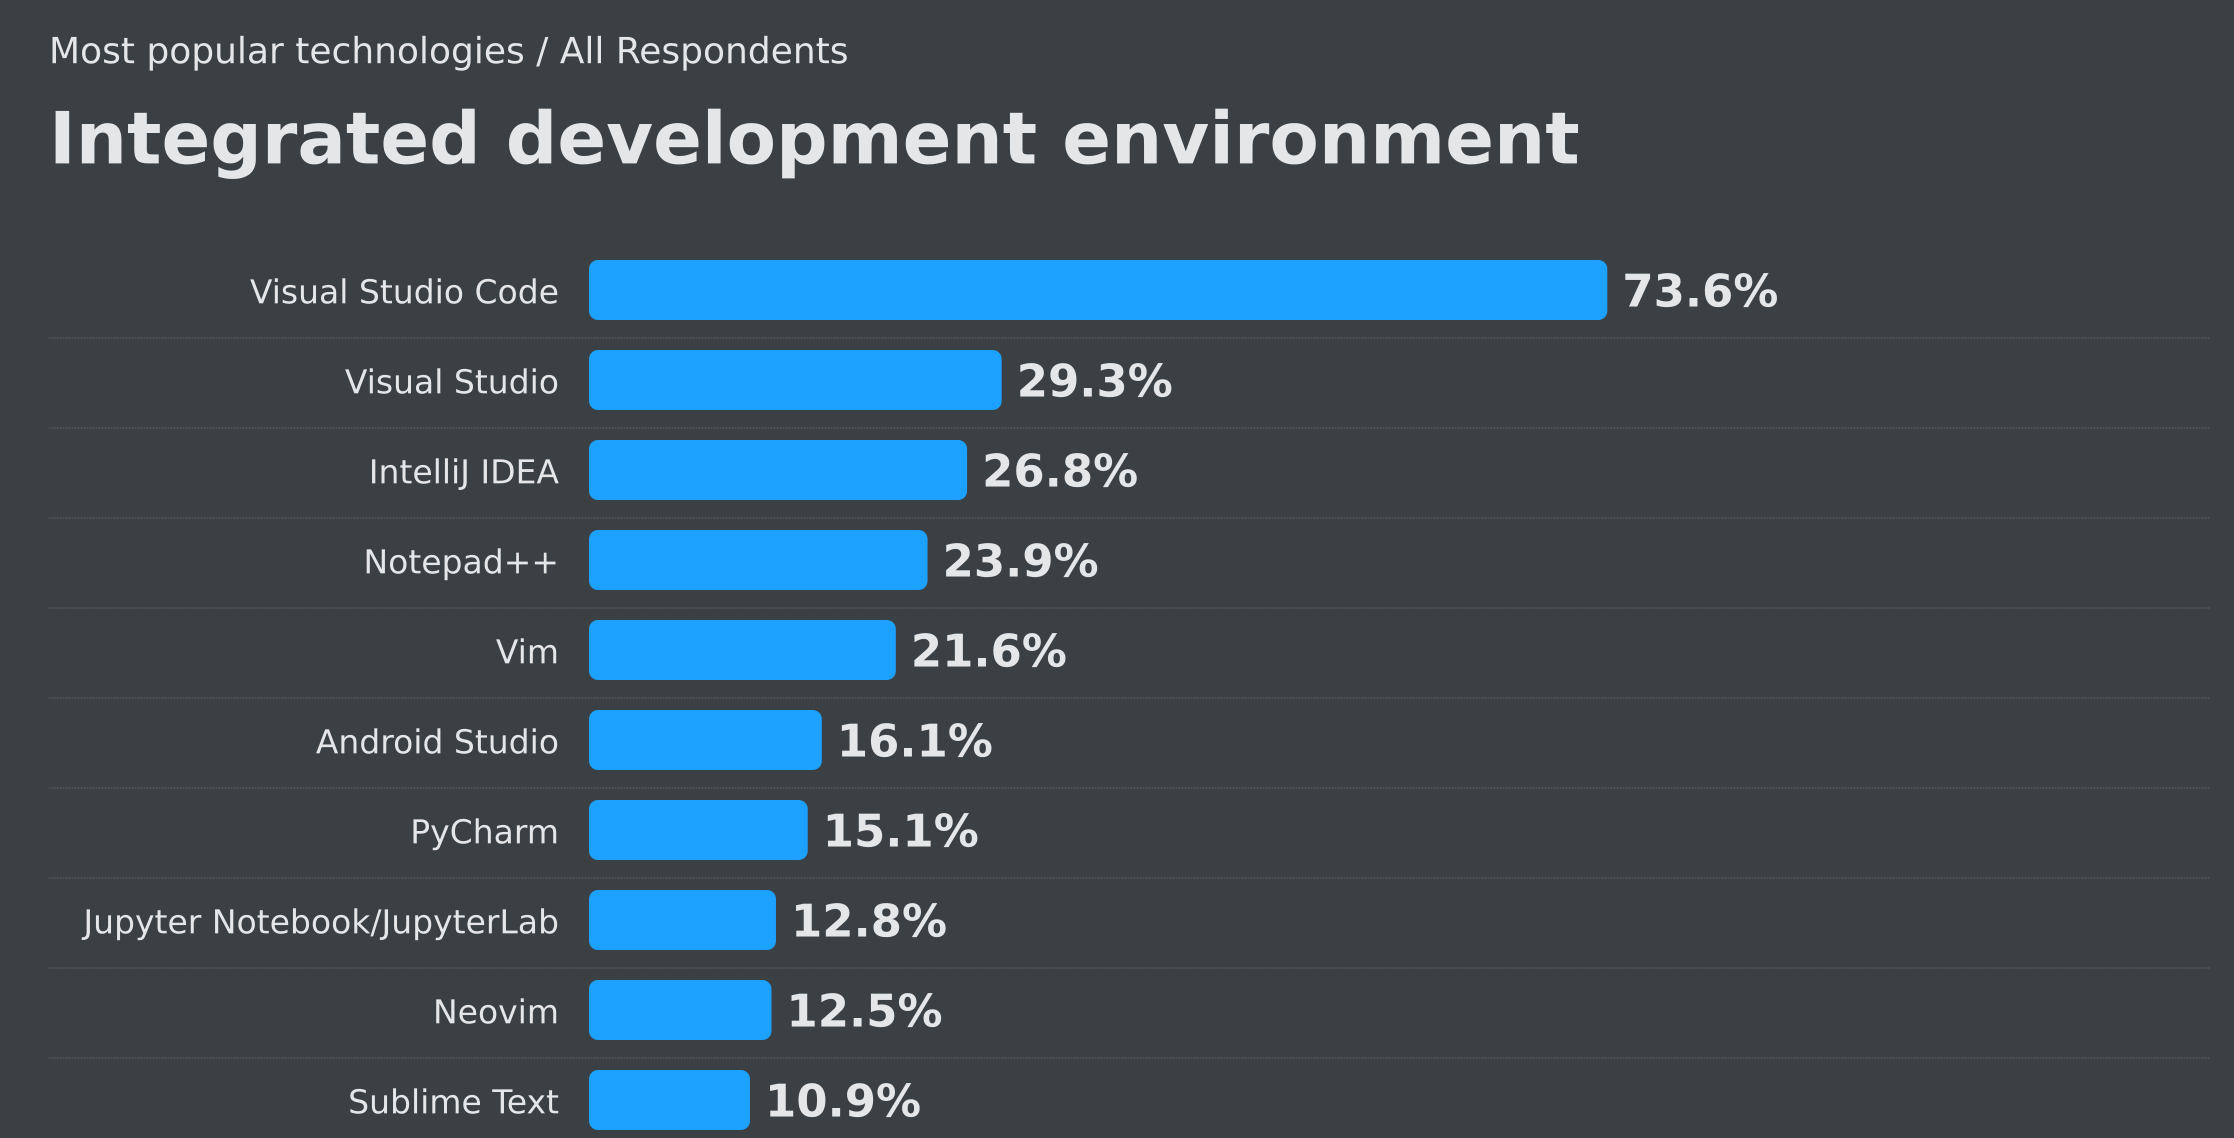
\includegraphics[width=.8\linewidth]{./pics/developersurvey2024.png}}{\scriptsize Source: \href{https://survey.stackoverflow.co/2024/charts/stackoverflow-dev-survey-2024-technology-most-popular-technologies-new-collab-tools-social.png}{https://survey.stackoverflow.co}}
	\caption{The most popular integrated development environments (IDEs) among developers, according to the 2024 Stack Overflow Developer Survey~\cite{stackoverflow2024}. Visual Studio Code is the highest ranking with 73.6\% usage, followed by Visual Studio and IntelliJ IDEA. All entries with less than 10\% popularity have been cut off, but can be viewed at the survey source.}
	\label{fig:stackoverflow-survey-result}
\end{figure}

A recent developer survey as can be seen in Figure~\ref{fig:stackoverflow-survey-result} indicates that Visual Studio Code is the most widely used IDE, with approximately twice as many users as Visual Studio, which holds the second position~\cite{stackoverflow2024}. IntelliJ IDEA ranks third in popularity. The preference for VS Code can be attributed to its lightweight nature, extensive extension marketplace, and strong integration with JavaScript and TypeScript ecosystems. This data supports the decision to prioritize VS Code support in the initial phases of Kipper's IDE integration strategy.

\section{Integration with other languages}
\setauthor{Luna Klatzer}

Kipper is not intended to function as a standalone language but is designed to integrate into modern web and server-side environments. By enabling developers to import and export generated modules in their preferred language—either JavaScript or TypeScript—the Kipper compiler allows for gradual adoption without necessitating a complete system overhaul or exclusive reliance on Kipper-generated code. This process also works the other way around, enabling libraries and existing code bases to be imported and utilised within Kipper projects. This would be supported through external module imports and a compatibility layer that adapts imports to Kipper's runtime features and type safety standards.

Due to its complexity, this functionality was not included in the scope of this paper but could be incrementally implemented once Kipper's core feature set is finalised and stabilised. By integrating import wrappers and code loaders into the Kipper compiler—capable of verifying the existence and integrity of external variables, functions, interfaces and classes—the compiler could enable seamless interoperability without compromising safety or disabling essential functionality to achieve direct one-to-one compatibility.

\section{Project Result \& Moving forward}
\setauthor{Luna Klatzer}

As of the time of writing, Kipper has met the initially defined objectives of this thesis but has not yet achieved a stable feature set or reached a v1.0 release. However, with the functionality outlined in this paper now implemented, the project will advance by refining and expanding upon the existing features to develop a language suitable for various scenarios and capable of bidirectional integration with its target environments.

While this thesis does not serve merely as a proof of concept, Kipper remains a closed-off project at this stage, lacking proper support for additional environments and much of the functionality expected from a fully developed modern programming language. However, the language will continue to be developed and extended with the long-term goal of establishing itself as a reliable programming language.

Furthermore, as an open-source project focused on all-round type safety and leveraging both \gls{transpilation} and the dynamic nature of an interpreter runtime, Kipper will continue to evolve and expand its feature set over the coming years, hoping to build support and grow as a project that can be utilised by a variety of developers.

%%% Local Variables:
%%% mode: LaTeX
%%% TeX-master: "../thesis"
%%% End:
